\documentclass[a4paper,12pt]{article}

\usepackage{estilos}

\pagestyle{empty}

\begin{document}
\begin{center}%
\begin{figure}[H]%
\begin{minipage}[H]{1\columnwidth}%
\centering%
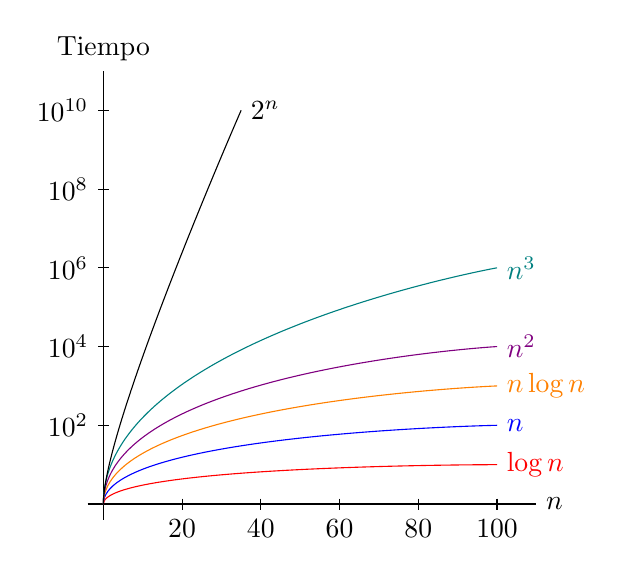
\begin{tikzpicture}

  \draw[] (-0.2,0) -- (5.5,0) node[right] {$n$};
  \draw[] (0,-0.2) -- (0,5.5) node[above] {Tiempo};

  \foreach \x/\xtext in {1/20, 2/40, 3/60, 4/80, 5/100}
  \draw[shift={(\x,0)}] (0pt,2pt) -- (0pt,-2pt) node[below] {$\xtext$};

  \foreach \y/\ytext in {1/10^2, 2/10^4, 3/10^6, 4/10^8, 5/10^{10}}
  \draw[shift={(0,\y)}] (2pt,0pt) -- (-2pt,0pt) node[left] {$\ytext$};

  \draw[red] (0,0)   .. controls +(up:.5cm) and +(left:0cm) .. (5,.5) node [right] {$\log n$};
  \draw[blue] (0,0)   .. controls +(up:.9cm) and +(left:0cm) .. (5,1) node [right] {$n$};
  \draw[orange] (0,0)   .. controls +(up:1.3cm) and +(left:0cm) .. (5,1.5) node [right] {$n \log n$};
  \draw[violet] (0,0)   .. controls +(up:1.7cm) and +(left:0cm) .. (5,2) node [right] {$n^2$};
  \draw[teal] (0,0)   .. controls +(up:2.1cm) and +(left:0cm) .. (5,3) node [right] {$n^3$};
  \draw[] (0,0)   .. controls +(up:1cm) and +(left:0cm) .. (1.75,5) node [right] {$2^n$};

\end{tikzpicture}
\caption{Representación gráfica de las tasas de crecimiento más frecuentes.}%
\end{minipage}%
\end{figure}%
\end{center}%
\end{document}
